\documentclass[a4paper,12pt]{article}
\usepackage[warn]{mathtext}
\usepackage[english, russian]{babel}

\usepackage[letterpaper,top=2cm,bottom=2cm,left=3cm,right=3cm,marginparwidth=1.75cm]{geometry}
\usepackage{amsmath}
\usepackage{graphicx}
\graphicspath{{pictures/}}
\DeclareGraphicsExtensions{.jpg}
\usepackage[colorlinks=true, allcolors=blue]{hyperref}

\title{Домашняя работа №1}
\author{A-05-19 Карпов Денис}
\date{}

\begin{document}
\maketitle

\section*{\Huge Задание №1}

\subsection*{Построить ДКА, распознающий описанный язык.}

\Large $1.\;L = {\{\omega \in \{a,b,c\}^*|\;|\omega|_c = 1\}}$\newline
Построим регулязное выражение, которое задаёт этот автомат:\newline
\Large$$a^*b^*ca^*b^*$$\newline
Построим на его основе ДКА:\newline
\begin{figure}[h]
\centering
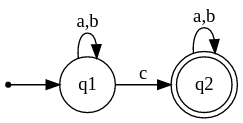
\includegraphics[scale=0.75]{1_1}
\end{figure}

\Large $2.\;L = {\{\omega \in \{a,b\}^*|\;|\omega|_a \le 2,\;|\omega|_b \ge 2\}}$\newline
Разделим описанный язык на $L_1$ и $L_2$, после чего, с помощью прямого произведения ДКА, построим конечный автомат.\newline
\Large $L_1 = {\{\omega \in \{a,b\}^*|\;|\omega|_a \le 2\}}$\newline
\Large $L_2 = {\{\omega \in \{a,b\}^*|\;|\omega|_b \ge 2\}}$\newline
Построим на их основе ДКА:\newline
\begin{figure}[h]
\centering
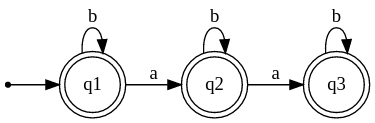
\includegraphics[scale=0.75]{1_2_1}
\caption{$L_1$}
\end{figure}

\begin{figure}[h]
\centering
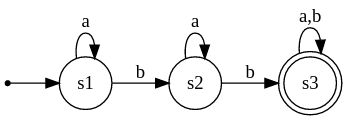
\includegraphics[scale=0.75]{1_2_2}
\caption{$L_2$}
\end{figure}

\begingroup
\raggedleft 
$A_1 = {\langle\sum_1 , Q_1, s_1, T_1, \delta_1 \rangle}$;
$A_2 = {\langle\sum_2 , Q_2, s_2, T_2, \delta_2 \rangle}$\newline
\endgroup
\begingroup
\raggedright 
$A = {\langle\sum , Q, s, T, \delta \rangle}$:
\begin{itemize}
\item $\sum = \sum_1 \cup \sum_2$
\item $Q = Q_1 \times Q_2$
\item $s = \langle s_1 , s_2\rangle$
\item $T = T_1 \times T_2$
\item $\delta(\langle q_1 , q_2\rangle, c) =  \langle \delta_1 (q_1 , c), \delta_2 (q_2, c) \rangle$
\end{itemize}
$\sum = \{q_1, q_2, q_3, s_1, s_2, s_3\}$\newline
\normalsize $Q = \{\langle q_1 , s_1 \rangle ,\langle q_1 , s_2 \rangle ,\langle q_1 , s_3 \rangle , \langle q_2 , s_1 \rangle , \langle q_2 , s_2 \rangle , \langle q_2 , s_3 \rangle , \langle q_3 , s_1 \rangle , \langle q_3 , s_2 \rangle , \langle q_3 , s_3 \rangle \}$\newline
\Large $s = \langle q_1 , s_1 \rangle$\newline
$T = \{\langle q_1 , s_3 \rangle ,\langle q_2 , s_3 \rangle ,\langle q_3 , s_3 \rangle\}$\newline
\begin{center}
\begin{tabular}{ |c|c|c| } 
\hline
  & a & b \\ [0.5ex] 
 \hline
 $\langle q_1 , s_1 \rangle$ & $\langle q_2 , s_1 \rangle$ & $\langle q_1 , s_2 \rangle$ \\ 
 $\langle q_1 , s_2 \rangle $ & $\langle q_2 , s_2 \rangle$ & $\langle q_1 , s_3 \rangle$ \\ 
 $\langle q_1 , s_3 \rangle $ & $\langle q_2 , s_3 \rangle$ & $\langle q_1 , s_3 \rangle$ \\ 
 $\langle q_2 , s_1 \rangle $ & $\langle q_3 , s_1 \rangle$ & $\langle q_2 , s_2 \rangle$ \\ 
 $\langle q_2 , s_2 \rangle $ & $\langle q_3 , s_2 \rangle$ & $\langle q_2 , s_3 \rangle$ \\
 $\langle q_2 , s_3 \rangle $ & $\langle q_3 , s_3 \rangle$ & $\langle q_2 , s_3 \rangle$ \\
 $\langle q_3 , s_1 \rangle $ &  & $\langle q_3 , s_2 \rangle$ \\
 $\langle q_3 , s_2 \rangle $ &  & $\langle q_3 , s_3 \rangle$ \\
 $\langle q_3 , s_3 \rangle $ &  & $\langle q_3 , s_3 \rangle$ \\
 \hline
\end{tabular}
\end{center}
\endgroup
Итоговый ДКА:\newline
\begin{figure}[h]
\centering
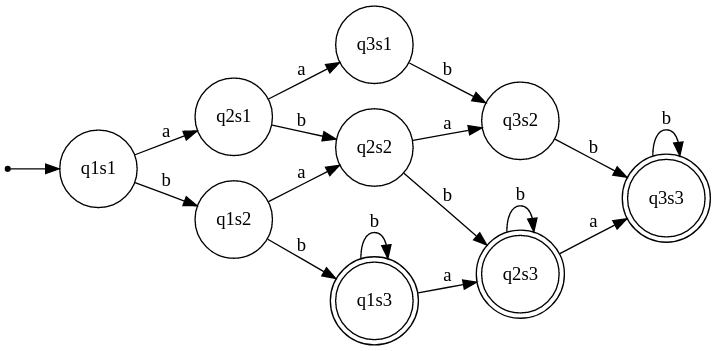
\includegraphics[scale=0.6]{1_2_3}
\end{figure}\newline
$3.\;L = {\{\omega \in \{a,b\}^*|\;|\omega|_a \ne |\omega|_b\}}$\newline
Если $L$ регулярный язык, то и $\overline{\rm L} = {\{\omega \in \{a,b\}^*|\;|\omega|_a = |\omega|_b\}}$.\newline
Докажем, что $\overline{\rm L} = {\{\omega \in \{a,b\}^*|\omega = a^nb^n\}}$ не является регурным, для этого воспользуемся леммой о разрастании.
Найдутся такие три слова, что $\omega = xyz, y \ne \lambda, |xy|\leq n \Rightarrow x = a^i, y = a^j, i+j \leq n, z = a^{n-i-j}+a^n=a^{2n}$. Пусть $k=0 \Rightarrow xy^0z=a^ia^{n-i-j}\ne a^n$, так как $j > 0 \Rightarrow$ язык не является регулярным. \newline
\newline$4.\;L = {\{\omega \in \{a,b\}^*|\;\omega\omega = \omega\omega\omega \}}$\newline
Данный язык представляется исключительно пустым словом: \newline
\begin{figure}[h]
\centering
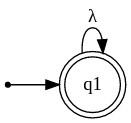
\includegraphics[scale=0.75]{1_4}
\end{figure}\newline

\section*{\Huge Задание №2}
\subsection*{Построить ДКА, распознающий описанный язык, построенный при помощи прямого произведения ДКА и его свойств.}
\Large $1.\;L = {\{\omega \in \{a,b\}^*|\;|\omega|_a \ge 2,\;|\omega|_b \ge 2\}}$\newline
Разделим описанный язык на $L_1$ и $L_2$, после чего, с помощью прямого произведения ДКА, построим конечный автомат.\newline
\Large $L_1 = {\{\omega \in \{a,b\}^*|\;|\omega|_a \ge 2\}}$\newline
\Large $L_2 = {\{\omega \in \{a,b\}^*|\;|\omega|_b \ge 2\}}$\newline
Построим на их основе ДКА:\newline
\begin{figure}[h]
\centering
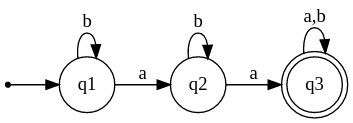
\includegraphics[scale=0.75]{2_1_1}
\caption{$L_1$}
\end{figure}
\begin{figure}[h]
\centering
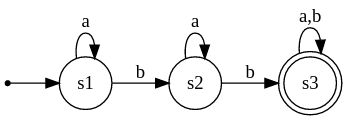
\includegraphics[scale=0.75]{2_1_2}
\caption{$L_2$}
\end{figure}\newline
\begingroup
\raggedleft 
$A_1 = {\langle\sum_1 , Q_1, s_1, T_1, \delta_1 \rangle}$;
$A_2 = {\langle\sum_2 , Q_2, s_2, T_2, \delta_2 \rangle}$\newline
\endgroup
\begingroup
\raggedright 
$A = {\langle\sum , Q, s, T, \delta \rangle}$:
\begin{itemize}
\item $\sum = \sum_1 \cup \sum_2$
\item $Q = Q_1 \times Q_2$
\item $s = \langle s_1 , s_2\rangle$
\item $T = T_1 \times T_2$
\item $\delta(\langle q_1 , q_2\rangle, c) =  \langle \delta_1 (q_1 , c), \delta_2 (q_2, c) \rangle$
\end{itemize}
$\sum = \{q_1, q_2, q_3, s_1, s_2, s_3\}$\newline
\normalsize $Q = \{\langle q_1 , s_1 \rangle ,\langle q_1 , s_2 \rangle ,\langle q_1 , s_3 \rangle , \langle q_2 , s_1 \rangle , \langle q_2 , s_2 \rangle , \langle q_2 , s_3 \rangle , \langle q_3 , s_1 \rangle , \langle q_3 , s_2 \rangle , \langle q_3 , s_3 \rangle \}$\newline
\Large $s = \langle q_1 , s_1 \rangle$\newline
$T = \langle q_3 , s_3 \rangle$\newline
\begin{center}
\begin{tabular}{ |c|c|c| } 
\hline
  & a & b \\ [0.5ex] 
 \hline
 $\langle q_1 , s_1 \rangle$ & $\langle q_2 , s_1 \rangle$ & $\langle q_1 , s_2 \rangle$ \\ 
 $\langle q_1 , s_2 \rangle $ & $\langle q_2 , s_2 \rangle$ & $\langle q_1 , s_3 \rangle$ \\ 
 $\langle q_1 , s_3 \rangle $ & $\langle q_2 , s_3 \rangle$ & $\langle q_1 , s_3 \rangle$ \\ 
 $\langle q_2 , s_1 \rangle $ & $\langle q_3 , s_1 \rangle$ & $\langle q_2 , s_2 \rangle$ \\ 
 $\langle q_2 , s_2 \rangle $ & $\langle q_3 , s_2 \rangle$ & $\langle q_2 , s_3 \rangle$ \\
 $\langle q_2 , s_3 \rangle $ & $\langle q_3 , s_3 \rangle$ & $\langle q_2 , s_3 \rangle$ \\
 $\langle q_3 , s_1 \rangle $ & $\langle q_3 , s_1 \rangle$ & $\langle q_3 , s_2 \rangle$ \\
 $\langle q_3 , s_2 \rangle $ & $\langle q_3 , s_2 \rangle$ & $\langle q_3 , s_3 \rangle$ \\
 $\langle q_3 , s_3 \rangle $ & $\langle q_3 , s_3 \rangle$ & $\langle q_3 , s_3 \rangle$ \\
 \hline
\end{tabular}
\end{center}
\endgroup
\begingroup
\raggedright 
Итоговый ДКА: \newline
\begin{figure}[h]
\centering
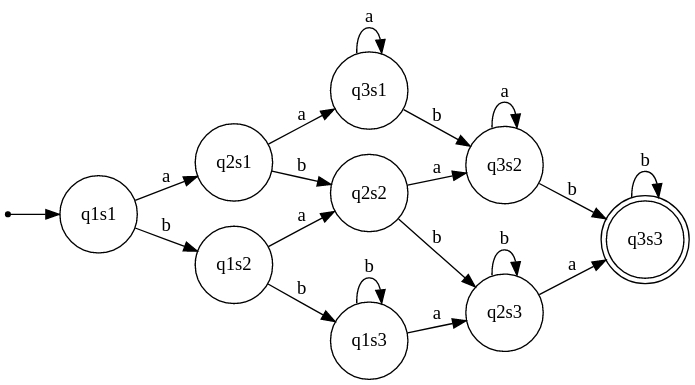
\includegraphics[scale=0.6]{2_1}
\end{figure}\newline
\endgroup
\Large $2.\;L = {\{\omega \in \{a,b\}^*|\;|\omega| \ge 3,\;|\omega| \; \text{нечётное}\}}$\newline
Разделим описанный язык на $L_1$ и $L_2$, после чего, с помощью прямого произведения ДКА, построим конечный автомат.\newline
\Large $L_1 = {\{\omega \in \{a,b\}^*|\;|\omega| \ge 3\}}$\newline
\Large $L_2 = {\{\omega \in \{a,b\}^*|\;|\omega| \text{ нечётное} \}}$\newline
Построим на их основе ДКА:\newline
\begin{center}
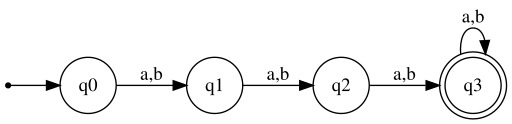
\includegraphics[width=0.75\textwidth]{2_2_1}\newline
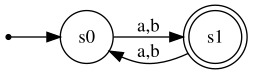
\includegraphics[width=0.5\textwidth]{2_2_2}\newline
\end{center}
$A_1 = {\langle\sum_1 , Q_1, s_1, T_1, \delta_1 \rangle}$;
$A_2 = {\langle\sum_2 , Q_2, s_2, T_2, \delta_2 \rangle}$\newline
$A = {\langle\sum , Q, s, T, \delta \rangle}$:
\begin{itemize}
\item $\sum = \sum_1 \cup \sum_2$
\item $Q = Q_1 \times Q_2$
\item $s = \langle s_1 , s_2\rangle$
\item $T = T_1 \times T_2$
\item $\delta(\langle q_1 , q_2\rangle, c) =  \langle \delta_1 (q_1 , c), \delta_2 (q_2, c) \rangle$
\end{itemize}
$\sum = \{q_0, q_1, q_2, q_3, s_0, s_1\}$\newline
\normalsize $Q = \{\langle q_0 , s_0 \rangle ,\langle q_0 , s_1 \rangle ,\langle q_1 , s_0 \rangle , \langle q_1 , s_1 \rangle , \langle q_2 , s_0 \rangle , \langle q_2 , s_1 \rangle , \langle q_3 , s_0 \rangle , \langle q_3 , s_1 \rangle\}$\newline
\Large $s = \langle q_0 , s_0 \rangle$\newline
$T = \langle q_3 , s_1 \rangle$\newline
\begin{center}
\begin{tabular}{ |c|c|c| } 
\hline
  & a & b \\ [0.5ex] 
 \hline
 $\langle q_0 , s_0 \rangle$ & $\langle q_1 , s_1 \rangle$ & $\langle q_1 , s_1 \rangle$ \\ 
 $\langle q_0 , s_1 \rangle $ & $\langle q_1 , s_0 \rangle$ & $\langle q_1 , s_0 \rangle$ \\ 
 $\langle q_1 , s_0 \rangle $ & $\langle q_2 , s_1 \rangle$ & $\langle q_2 , s_1 \rangle$ \\ 
 $\langle q_1 , s_1 \rangle $ & $\langle q_2 , s_0 \rangle$ & $\langle q_2 , s_0 \rangle$ \\ 
 $\langle q_2 , s_0 \rangle $ & $\langle q_3 , s_1 \rangle$ & $\langle q_3 , s_1 \rangle$ \\
 $\langle q_2 , s_1 \rangle $ & $\langle q_3 , s_0 \rangle$ & $\langle q_3 , s_0 \rangle$ \\
 $\langle q_3 , s_0 \rangle $ & $\langle q_3 , s_1 \rangle$ & $\langle q_3 , s_1 \rangle$ \\
 $\langle q_3 , s_1 \rangle $ & $\langle q_3 , s_0 \rangle$ & $\langle q_3 , s_0 \rangle$ \\
 \hline
\end{tabular}
\end{center}
Итоговый ДКА:
\begin{center}
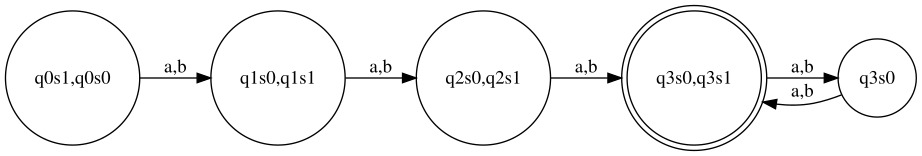
\includegraphics[width=1.15\textwidth]{2_2}\newline
\end{center}
\Large $3.\;L = {\{\omega \in \{a,b\}^*|\;|\omega|_a \text{чётно}\land|\omega|_b \; \text{кратно трём}\}}$\newline
Разделим описанный язык на $L_1$ и $L_2$, после чего, с помощью прямого произведения ДКА, построим конечный автомат.\newline
\Large $L_1 = {\{\omega \in \{a,b\}^*|\;|\omega|_a \text{чётно}\}}$\newline
\Large $L_2 = {\{\omega \in \{a,b\}^*|\;|\omega|_b \; \text{кратно трём}\}}$\newline
Построим на их основе ДКА:\newline
\begin{center}
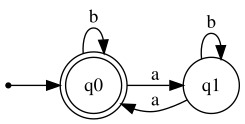
\includegraphics[width=0.5\textwidth]{2_3_1}\newline
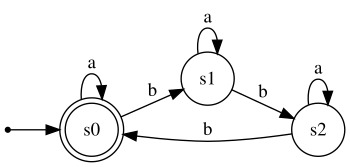
\includegraphics[width=0.75\textwidth]{2_3_2}\newline
\end{center}
$A_1 = {\langle\sum_1 , Q_1, s_1, T_1, \delta_1 \rangle}$;
$A_2 = {\langle\sum_2 , Q_2, s_2, T_2, \delta_2 \rangle}$\newline
$A = {\langle\sum , Q, s, T, \delta \rangle}$:
\begin{itemize}
\item $\sum = \sum_1 \cup \sum_2$
\item $Q = Q_1 \times Q_2$
\item $s = \langle s_1 , s_2\rangle$
\item $T = T_1 \times T_2$
\item $\delta(\langle q_1 , q_2\rangle, c) =  \langle \delta_1 (q_1 , c), \delta_2 (q_2, c) \rangle$
\end{itemize}
$\sum = \{q_0, q_1, s_0, s_1, s_2\}$\newline
\normalsize $Q = \{\langle q_0 , s_0 \rangle ,\langle q_0 , s_1 \rangle ,\langle q_0 , s_2 \rangle , \langle q_1 , s_0 \rangle , \langle q_1 , s_1 \rangle , \langle q_1 , s_2 \rangle \}$\newline
\Large $s = \langle q_0 , s_0 \rangle$\newline
$T = \langle q_0 , s_0 \rangle$\newline
\begin{center}
\begin{tabular}{ |c|c|c| } 
\hline
  & a & b \\ [0.5ex] 
 \hline
 $\langle q_0 , s_0 \rangle $ & $\langle q_1 , s_0 \rangle$ & $\langle q_0 , s_1 \rangle$ \\ 
 $\langle q_0 , s_1 \rangle $ & $\langle q_1 , s_1 \rangle$ & $\langle q_0 , s_2 \rangle$ \\ 
 $\langle q_0 , s_2 \rangle $ & $\langle q_1 , s_2 \rangle$ & $\langle q_0 , s_0 \rangle$ \\ 
 $\langle q_1 , s_0 \rangle $ & $\langle q_0 , s_0 \rangle$ & $\langle q_1 , s_1 \rangle$ \\ 
 $\langle q_1 , s_1 \rangle $ & $\langle q_0 , s_1 \rangle$ & $\langle q_1 , s_2 \rangle$ \\
 $\langle q_1 , s_2 \rangle $ & $\langle q_0 , s_2 \rangle$ & $\langle q_1 , s_0 \rangle$ \\
 \hline
\end{tabular}
\end{center}
Итоговый ДКА:
\begin{center}
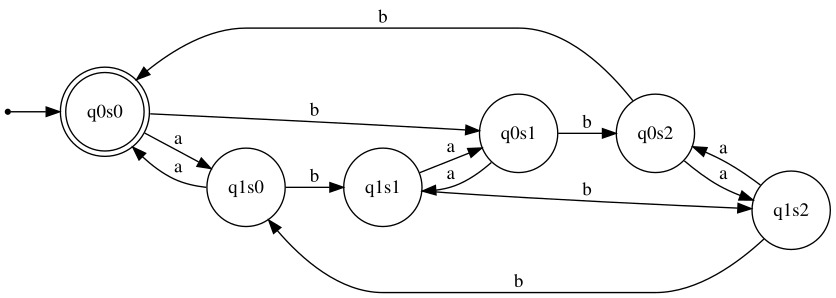
\includegraphics[width=1.15\textwidth]{2_3}\newline
\end{center}
\Large $4.\;L_4 = \overline{L_3}$\newline
$\overline{L} = {\langle\sum , Q, s, Q\setminus T, \delta \rangle}$\newline
$\sum = \{q_0, q_1, s_0, s_1, s_2\}$\newline
\normalsize $Q = \{\langle q_0 , s_0 \rangle ,\langle q_0 , s_1 \rangle ,\langle q_0 , s_2 \rangle , \langle q_1 , s_0 \rangle , \langle q_1 , s_1 \rangle , \langle q_1 , s_2 \rangle \}$\newline
\Large $s = \langle q_0 , s_0 \rangle$\newline
$T = \{\langle q_0 , s_1 \rangle ,\langle q_0 , s_2 \rangle , \langle q_1 , s_0 \rangle , \langle q_1 , s_1 \rangle , \langle q_1 , s_2 \rangle \}$\newline
Итоговый ДКА:
\begin{center}
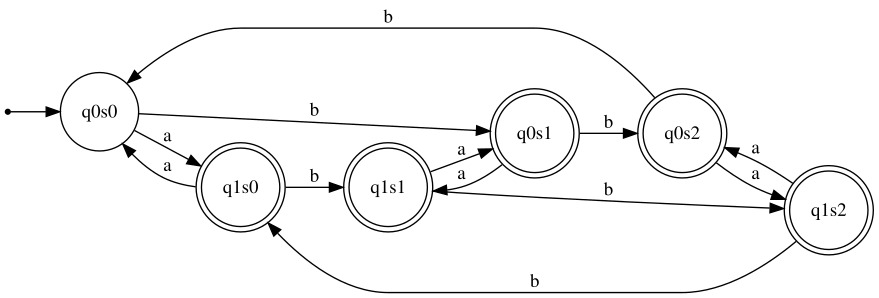
\includegraphics[width=1.15\textwidth]{2_4}\newline
\end{center}
$5.\;L_5 = L_2 \setminus L_3$\newline
\Large $L_5 = L_2 \cap \overline{L_3}$\newline
Переименуем вершины в ДКА из прошлых пунктов:
$A_1 = {\langle\sum_1 , Q_1, s_1, T_1, \delta_1 \rangle}$;
$A_2 = {\langle\sum_2 , Q_2, s_2, Q_2 \setminus T_2, \delta_2 \rangle}$\newline
$A = {\langle\sum , Q, s, T, \delta \rangle}$:
\begin{itemize}
\item $\sum = \sum_1 \cup \sum_2$
\item $Q = Q_1 \times Q_2$
\item $s = \langle s_1 , s_2\rangle$
\item $T = T_1 \times (Q_2 \setminus T_2)$
\item $\delta(\langle q_1 , q_2\rangle, c) =  \langle \delta_1 (q_1 , c), \delta_2 (q_2, c) \rangle$
\end{itemize}
$\sum = \{q_0, q_1, q_2, q_3, q_4, s_0, s_1, s_2, s_3, s_4, s_5\}$\newline
\normalsize $Q = \{\langle q_0 , s_0 \rangle ,\langle q_0 , s_1 \rangle ,\langle q_0 , s_2 \rangle , \langle q_0 , s_3 \rangle , \langle q_0 , s_4 \rangle , \langle q_0 , s_5 \rangle , \langle q_1 , s_0 \rangle , \langle q_1 , s_1 \rangle, \langle q_1 , s_2 \rangle, \langle q_1 , s_3 \rangle , \langle q_1 , s_4 \rangle , \langle q_1 , s_5 \rangle ,\newline \langle q_2 , s_0 \rangle , \langle q_2 , s_1 \rangle, \langle q_2 , s_2 \rangle, \langle q_2 , s_3 \rangle , \langle q_2 , s_4 \rangle , \langle q_2 , s_5 \rangle , \langle q_3 , s_0 \rangle , \langle q_3 , s_1 \rangle, \langle q_3 , s_2 \rangle, \langle q_3 , s_3 \rangle , \langle q_3 , s_4 \rangle , \langle q_3 , s_5 \rangle\, \newline \langle q_4 , s_0 \rangle , \langle q_4 , s_1 \rangle, \langle q_4 , s_2 \rangle, \langle q_4 , s_3 \rangle , \langle q_4 , s_4 \rangle , \langle q_4 , s_5 \rangle\}$\newline
\Large $s = \langle q_0 , s_0 \rangle$\newline
$T = \{\langle q_3 , s_1 \rangle ,\langle q_3 , s_2 \rangle , \langle q_3 , s_3 \rangle , \langle q_3 , s_4 \rangle , \langle q_3 , s_5 \rangle \}$\newline
\begin{center}
\begin{tabular}{ |c|c|c| } 
\hline
  & a & b \\ [0.5ex] 
 \hline
 $\langle q_0 , s_0 \rangle$ & $\langle q_1 , s_1 \rangle$ & $\langle q_1 , s_3 \rangle$ \\ 
 $\langle q_0 , s_1 \rangle$ & $\langle q_1 , s_0 \rangle$ & $\langle q_1 , s_2 \rangle$ \\
 $\langle q_0 , s_2 \rangle$ & $\langle q_1 , s_3 \rangle$ & $\langle q_1 , s_5 \rangle$ \\ 
 $\langle q_0 , s_3 \rangle$ & $\langle q_1 , s_2 \rangle$ & $\langle q_1 , s_4 \rangle$ \\
 $\langle q_0 , s_4 \rangle$ & $\langle q_1 , s_5 \rangle$ & $\langle q_1 , s_0 \rangle$ \\
 $\langle q_0 , s_5 \rangle$ & $\langle q_1 , s_4 \rangle$ & $\langle q_1 , s_1 \rangle$ \\ 
 $\langle q_1 , s_0 \rangle$ & $\langle q_2 , s_1 \rangle$ & $\langle q_2 , s_3 \rangle$ \\ 
 $\langle q_1 , s_1 \rangle$ & $\langle q_2 , s_0 \rangle$ & $\langle q_2 , s_2 \rangle$ \\
 $\langle q_1 , s_2 \rangle$ & $\langle q_2 , s_3 \rangle$ & $\langle q_2 , s_5 \rangle$ \\ 
 $\langle q_1 , s_3 \rangle$ & $\langle q_2 , s_2 \rangle$ & $\langle q_2 , s_4 \rangle$ \\
 $\langle q_1 , s_4 \rangle$ & $\langle q_2 , s_5 \rangle$ & $\langle q_2 , s_0 \rangle$ \\
 $\langle q_1 , s_5 \rangle$ & $\langle q_2 , s_4 \rangle$ & $\langle q_2 , s_1 \rangle$ \\ 
 $\langle q_2 , s_0 \rangle$ & $\langle q_3 , s_1 \rangle$ & $\langle q_3 , s_3 \rangle$ \\ 
 $\langle q_2 , s_1 \rangle$ & $\langle q_3 , s_0 \rangle$ & $\langle q_3 , s_2 \rangle$ \\
 $\langle q_2 , s_2 \rangle$ & $\langle q_3 , s_3 \rangle$ & $\langle q_3 , s_5 \rangle$ \\ 
 $\langle q_2 , s_3 \rangle$ & $\langle q_3 , s_2 \rangle$ & $\langle q_3 , s_4 \rangle$ \\
 $\langle q_2 , s_4 \rangle$ & $\langle q_3 , s_5 \rangle$ & $\langle q_3 , s_0 \rangle$ \\
 $\langle q_2 , s_5 \rangle$ & $\langle q_3 , s_4 \rangle$ & $\langle q_3 , s_1 \rangle$ \\ 
 $\langle q_3 , s_0 \rangle$ & $\langle q_4 , s_1 \rangle$ & $\langle q_4 , s_3 \rangle$ \\ 
 $\langle q_3 , s_1 \rangle$ & $\langle q_4 , s_0 \rangle$ & $\langle q_4 , s_2 \rangle$ \\
 $\langle q_3 , s_2 \rangle$ & $\langle q_4 , s_3 \rangle$ & $\langle q_4 , s_5 \rangle$ \\ 
 $\langle q_3 , s_3 \rangle$ & $\langle q_4 , s_2 \rangle$ & $\langle q_4 , s_4 \rangle$ \\
 $\langle q_3 , s_4 \rangle$ & $\langle q_4 , s_5 \rangle$ & $\langle q_4 , s_0 \rangle$ \\
 $\langle q_3 , s_5 \rangle$ & $\langle q_4 , s_4 \rangle$ & $\langle q_4 , s_1 \rangle$ \\ 
 $\langle q_4 , s_0 \rangle$ & $\langle q_3 , s_1 \rangle$ & $\langle q_3 , s_3 \rangle$ \\ 
 $\langle q_4 , s_1 \rangle$ & $\langle q_3 , s_0 \rangle$ & $\langle q_3 , s_2 \rangle$ \\
 $\langle q_4 , s_2 \rangle$ & $\langle q_3 , s_3 \rangle$ & $\langle q_3 , s_5 \rangle$ \\ 
 $\langle q_4 , s_3 \rangle$ & $\langle q_3 , s_2 \rangle$ & $\langle q_3 , s_4 \rangle$ \\
 $\langle q_4 , s_4 \rangle$ & $\langle q_3 , s_5 \rangle$ & $\langle q_3 , s_0 \rangle$ \\
 $\langle q_4 , s_5 \rangle$ & $\langle q_3 , s_4 \rangle$ & $\langle q_3 , s_1 \rangle$ \\ 
 \hline
\end{tabular}
\end{center}
С помощью таблицы переходов построим ДКА:
\begin{center}
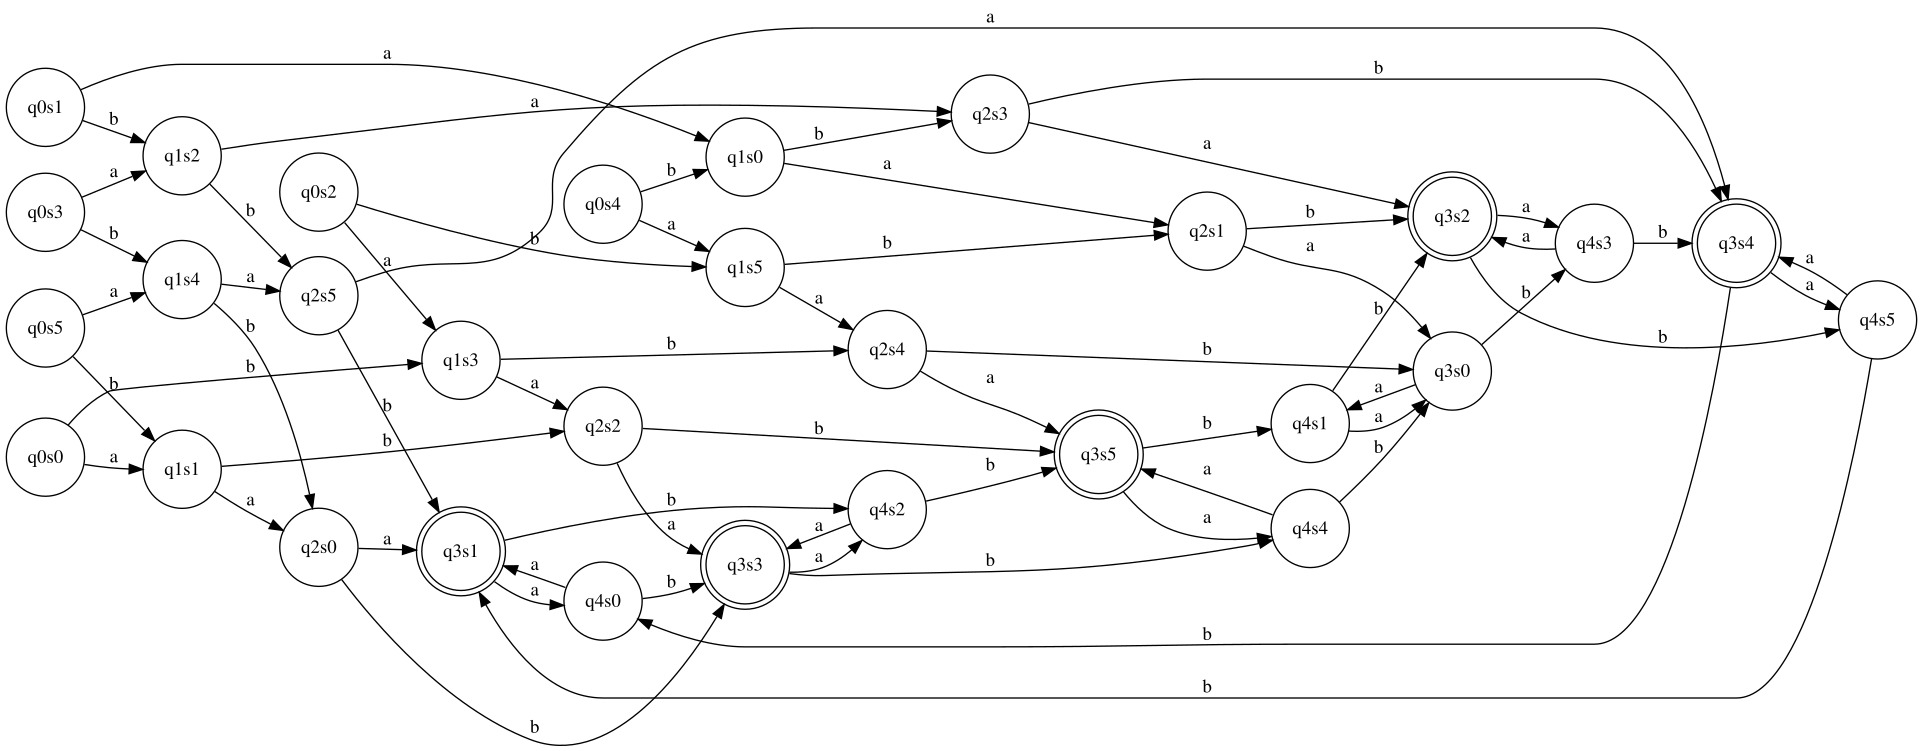
\includegraphics[width=1.15\textwidth]{2_5}\newline
\end{center}
Имеем несколько недостижимых состояний, избавимся от них.\newline
\begin{center}
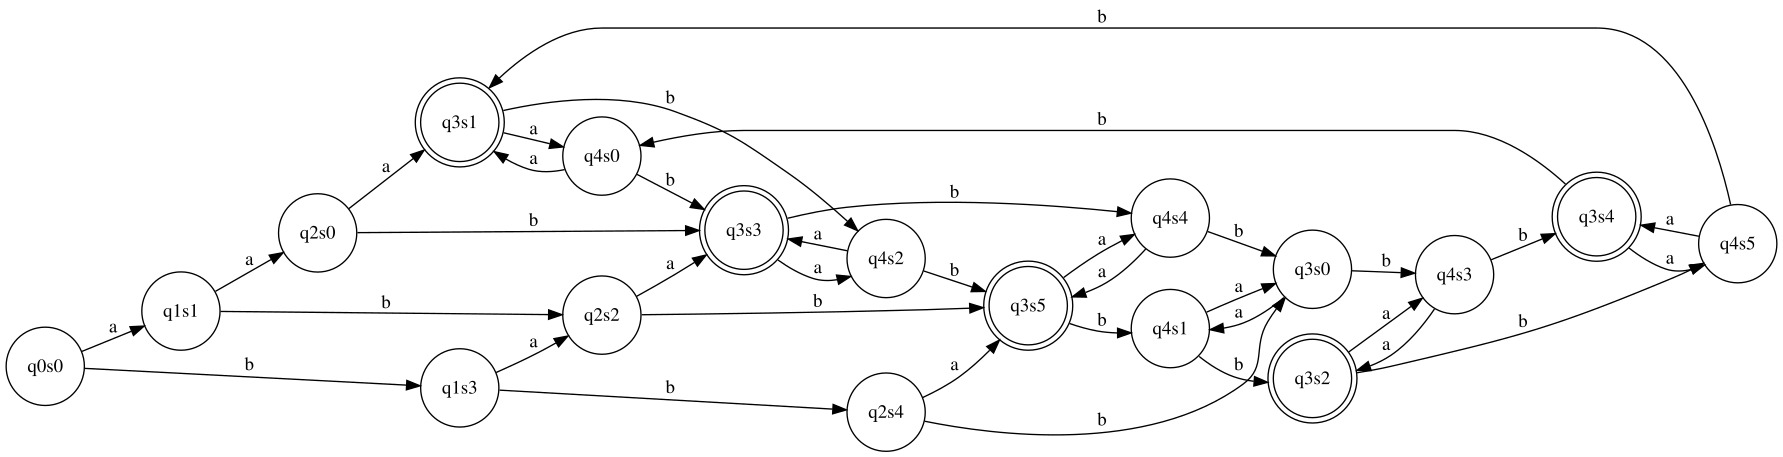
\includegraphics[width=1.15\textwidth]{2_5_1}\newline
\end{center}

\section*{\Huge Задание №3}
\subsection*{Построить минимальный ДКА по регулярному выражению.}
\Large $1.\;(ab+aba)^*a$\newline
Построим НКА:
\begin{center}
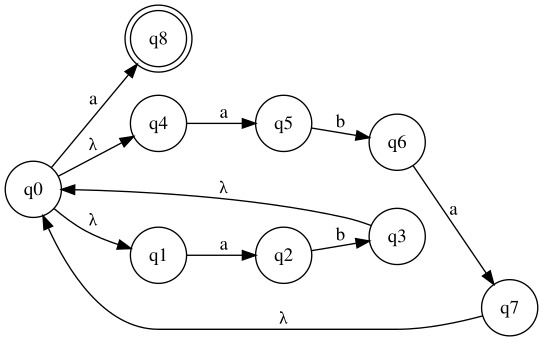
\includegraphics{3_1_nka}\newline
\end{center}
\begin{center}
\begin{tabular}{ |c|c|c| } 
\hline
  & a & b \\ [0.5ex] 
 \hline
$q0$ & $q2q5q8$ & $\emptyset$ \\
$q2q5q8$ & $\emptyset$ & $q3q6$ \\
$q3q6$ & $q2q5q7q8$ & $\emptyset$ \\
$q2q5q7q8$ & $q2q5q8$ & $q3q6$ \\
 \hline
\end{tabular}
\end{center}
Итоговый ДКА:
\begin{center}
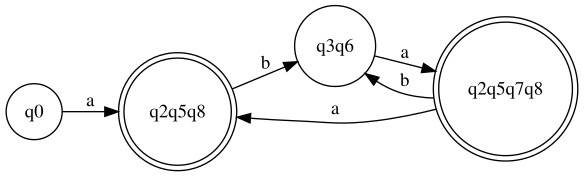
\includegraphics{3_1}\newline
\end{center}
\Large $2.\;a(a(ab)^*b)^*(ab)^*$\newline
Построим НКА:
\begin{center}
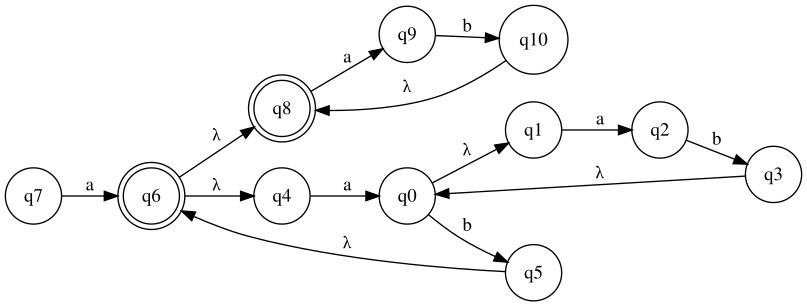
\includegraphics[width=1.15\textwidth]{3_2_nka}\newline
\end{center}
\begin{center}
\begin{tabular}{ |c|c|c| } 
\hline
  & a & b \\ [0.5ex] 
 \hline
$q7$ & $q6$ & $\emptyset$ \\
$q6$ & $q0q9$ & $\emptyset$ \\
$q0q9$ & $q2$ & $q5q10$ \\
$q2$ & $\emptyset$ & $q3$ \\
$q3$ & $q2$ & $q5$ \\
$q5$ & $q0q9$ & $\emptyset$ \\
$q5q10$ & $q0q9$ & $\emptyset$ \\
 \hline
\end{tabular}
\end{center}
Полученный ДКА:
\begin{center}
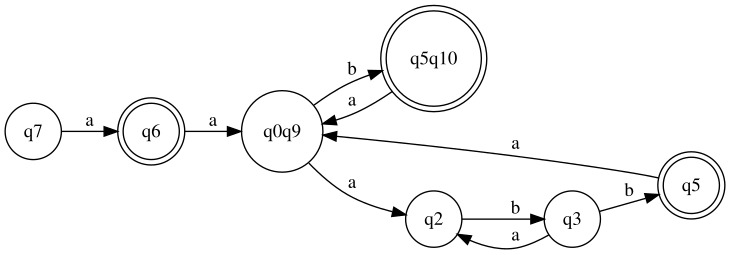
\includegraphics[width=1.15\textwidth]{3_2}\newline
\end{center}
Попробуем минимизировать получившийся ДКА:\newline
$\text{0 эквивалентность:} \; I_0=\{q7,q0q9,q2,q3\},I_1=\{q5,q5q10,q6\}$
$\text{1 эквивалентность:} \; I_2=\{q7\},I_3=\{q0q9,q3\},I_4=\{q2\},I_1=\{q5,q5q10,q6\}$\newline
Это конечный результат сегментации, так как не представляется возможным разделить по эквивалентностям.
Итоговый ДКА:
\begin{center}
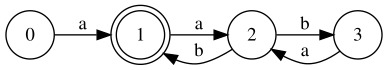
\includegraphics[width=0.75\textwidth]{3_2_1}\newline
\end{center}
\Large $3.\;(a+(a+b)(a+b)b)^*$\newline
Построим НКА:
\begin{center}
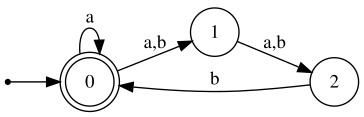
\includegraphics[width=0.5\textwidth]{3_3_nka}\newline
\end{center}
\begin{center}
\begin{tabular}{ |c|c|c| } 
\hline
  & a & b \\ [0.5ex] 
 \hline
$0$ & $01$ & $1$ \\
$1$ & $2$ & $2$ \\
$01$ & $012$ & $12$ \\
$012$ & $012$ & $012$ \\
$12$ & $2$ & $02$ \\
$2$ & $\emptyset$ & $0$ \\
$02$ & $01$ & $01$ \\
 \hline
\end{tabular}
\end{center}
Полученный ДКА:
\begin{center}
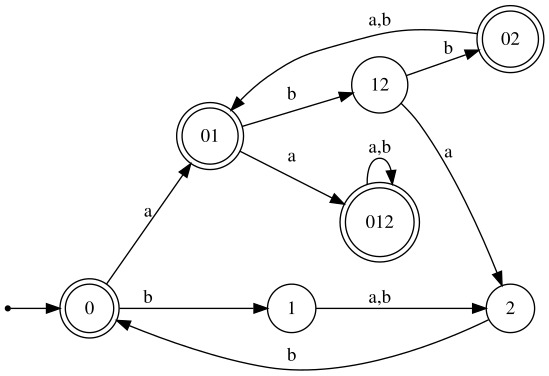
\includegraphics[width=1.15\textwidth]{3_3}\newline
\end{center}
После 3 эквивалентности можем сделать вывод, что ДКА выше -- минимальный.\newline
\Large $4.\;(b+c)((ab)^*c+(ba)^*)^*$\newline
Построим НКА:
\begin{center}
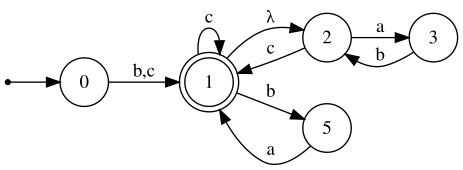
\includegraphics[width=0.65\textwidth]{3_4_nka}\newline
\end{center}
\begin{center}
\begin{tabular}{ |c|c|c|c| } 
\hline
  & a & b & c \\ [0.5ex] 
 \hline
$0$ & $\emptyset$ & $1$ & $1$ \\
$1$ & $3$ & $5$ & $1$ \\
$3$ & $\emptyset$ & $2$ & $\emptyset$ \\
$5$ & $1$ & $\emptyset$ & $\emptyset$ \\
$2$ & $3$ & $\emptyset$ & $1$ \\
 \hline
\end{tabular}
\end{center}
Полученный ДКА:
\begin{center}
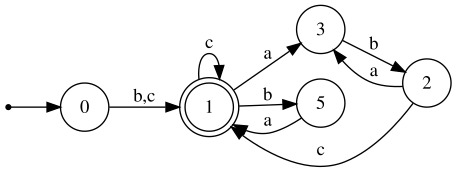
\includegraphics[width=0.65\textwidth]{3_4}\newline
\end{center}
Данный автомат является минимальным.\newline
\Large $5.\;(a+b)^+(aa+bb+abab+baba)(a+b)^+$\newline
Построим НКА:
\begin{center}
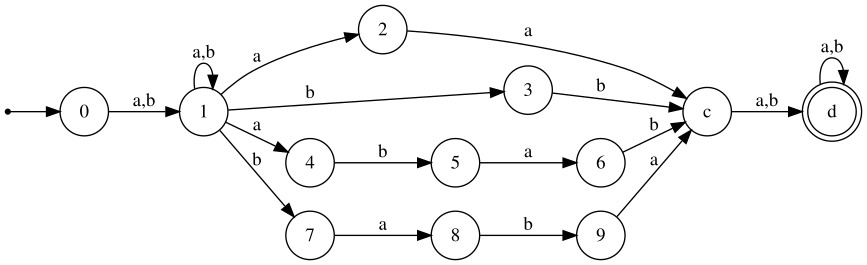
\includegraphics[width=1\textwidth]{3_5_nka}\newline
\end{center}
\begin{center}
\begin{tabular}{ |c|c|c| } 
\hline
  & a & b \\ [0.5ex] 
 \hline
$0$ & $1$ & $1$ \\
$1$ & $124$ & $137$ \\
$124$ & $124c$ & $1357$ \\
$137$ & $1248$ & $137c$ \\
$124c$ & $124cd$ & $1357d$ \\
$1357$ & $12468$ & $137c$ \\
$1248$ & $124c$ & $13579$ \\
$137c$ & $1248d$ & $137cd$ \\
$124cd$ & $124cd$ & $1357d$ \\
$1357d$ & $12468d$ & $137cd$ \\
$12468$ & $124c$ & $13579c$ \\
$13579$ & $12468c$ & $137c$ \\
$1248d$ & $124cd$ & $13579d$ \\
$137cd$ & $1248d$ & $137cd$ \\
$12468d$ & $124cd$ & $13579cd$ \\
$13579c$ & $12468cd$ & $137cd$ \\
$12468c$ & $124cd$ & $13579cd$ \\
$13579d$ & $12468cd$ & $137cd$ \\
$13579cd$ & $12468cd$ & $137cd$ \\
$12468cd$ & $124cd$ & $13579cd$ \\
 \hline
\end{tabular}
\end{center}
Полученный ДКА:
\begin{center}
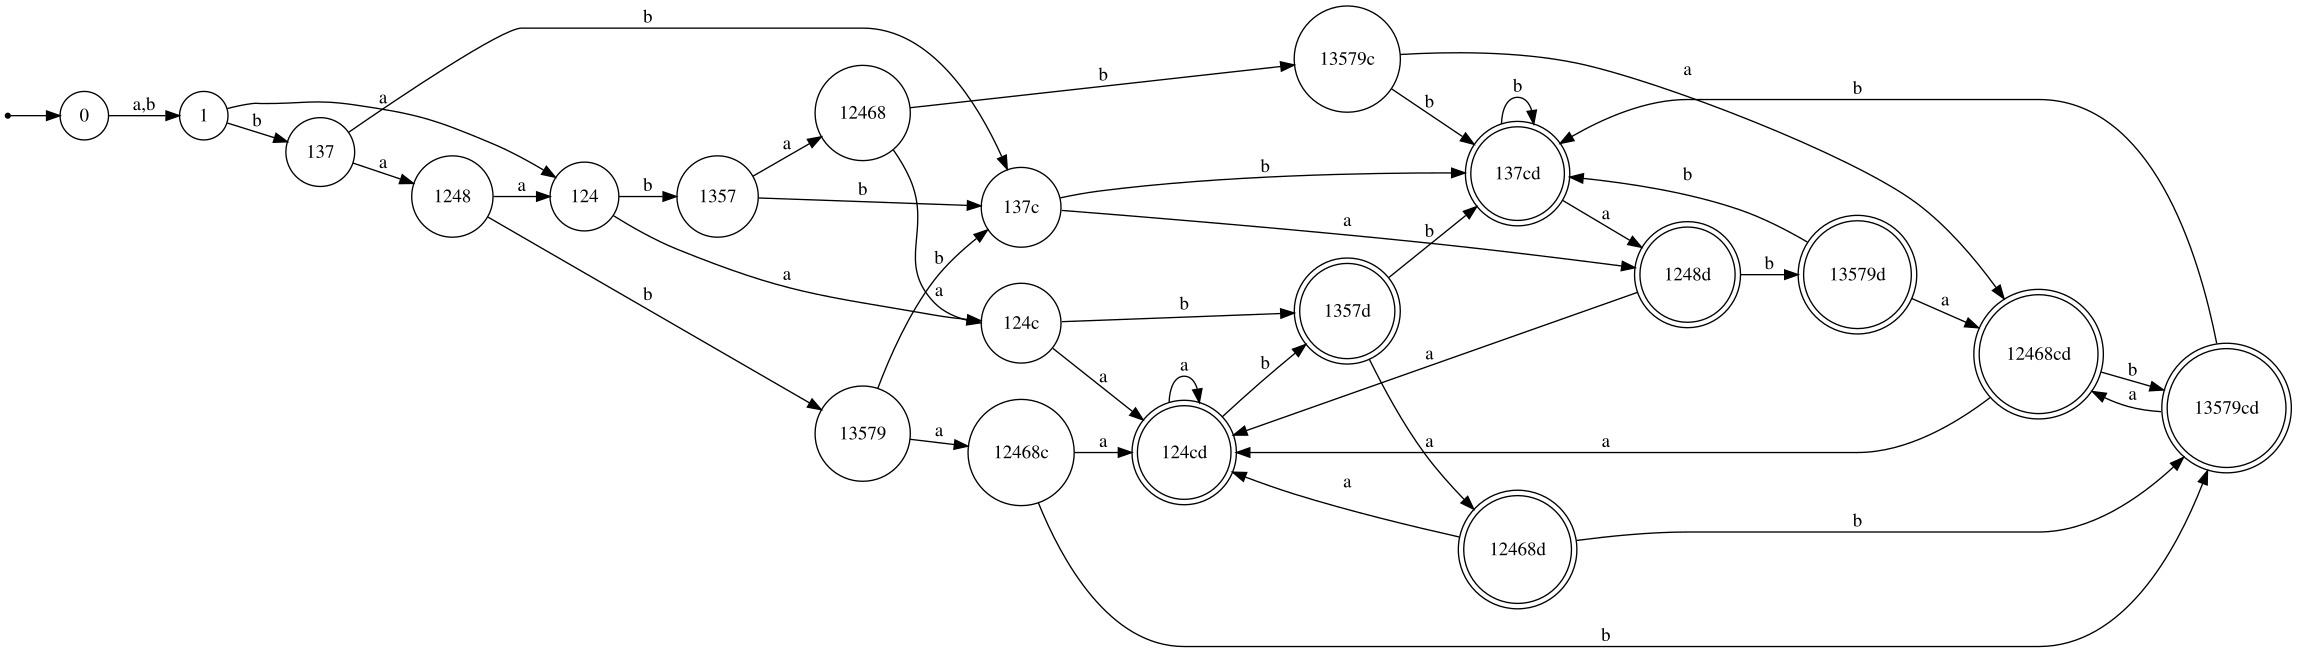
\includegraphics[width=1.15\textwidth]{3_5}\newline
\end{center}
Попробуем минимизировать получившийся ДКА:\newline
$\text{0 эквивалентность:} \; I_0=\{0,1,137,1248,124,1357,13579,12468,\newline 124c,137c,12468c,13579c\},I_1=\{124cd,1357d,137cd,12468d, \newline
1248d,13579d,12468cd,13579cd\}$\newline
$\text{1 эквивалентность:} \; I_1; I_2=\{0,1,137,124,1248,1357,13579,12468\},\newline I_3=\{124c,137c,12468c,13579c\}$\newline
$\text{2 эквивалентность:} \; I_1; I_3; I_4=\{0,1,1248\}, I_5=\{137, 1357\}, 
I_6=\{124\}, I_7=\{13579, 12468\}\newline$
$\text{3 эквивалентность:} \; I_1; I_3; I_6; I_7; I_8=\{0\}, I_9=\{1\}, 
I_{10}=\{1248\}, I_{11}=\{137\},I_{12}=\{1357\}\newline$
Это конечный результат сегментации, так как не представляется возможным разделить по эквивалентностям.
Итоговый ДКА:
\begin{center}
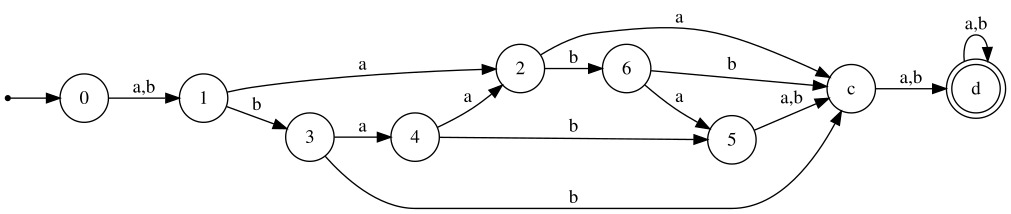
\includegraphics[width=1.15\textwidth]{3_5_1}\newline
\end{center}

\section*{\Huge Задание №4}
\subsection*{Определить является ли языкрегулярным или нет.}
\Large $1.\;L = \{(aab)^nb(aba)^m|n \ge 0, m \ge 0\}$\newline
Так как n и m не зависят друг от друга, то мы можем представить язык следующим регулярным выражением: \newline $(aab)^*b(aba)^*$. Построим ДКА:
\begin{center}
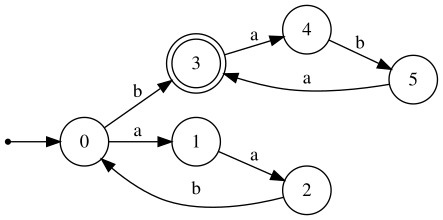
\includegraphics[width=1.15\textwidth]{4_1}\newline
\end{center}
\Large $2.\;L = \{uaav|u \in \{a,b\}^*, v \in \{a,b\}^*, |u|_b \ge |v|_a\}$\newline
Пусть $\exists$ слово $\omega = b^naaa^n \in L$.  
Найдутся такие три слова, что $\omega = xyz, y \ne \lambda, |xy|\leq n \Rightarrow x = b^i, y = b^j, i+j \leq n, z = b^{n-i-j}aaa^n$. Пусть $k=0 \Rightarrow xy^0z=b^ib^{n-i-j}aaa^n = b^{n-j}aaa^n \notin L$, так как $j \ne 0$, то есть язык не является регулярным. \newline
\Large $3.\;L = \{a^m\omega|\omega \in \{a,b\}^*, 1 \le |\omega|_b \le m\}$\newline
Пусть $\exists$ слово $\psi = a^nb^n \in L$.  
Найдутся такие три слова, что $\psi = xyz, y \ne \lambda, |xy|\leq n \Rightarrow x = a^i, y = a^j, i+j \leq n, z = a^{n-i-j}b^n$. Пусть $k=0 \Rightarrow xy^0z=a^ia^{n-i-j}b^n = a^{n-j}b^n \notin L$, так как $j \ne 0$, то есть язык не является регулярным. \newline
\Large $4.\;L = \{a^kb^ma^n|k = n \vee m > 0\}$\newline
Пусть $\exists$ слово $\omega = a^nba^n \in L$.  
Найдутся такие три слова, что $\omega = xyz, y \ne \lambda, |xy|\leq n \Rightarrow x = a^i, y = a^j, i+j \leq n, z = a^{n-i-j}ba^n$. Пусть $k=0 \Rightarrow xy^0z=a^ia^{n-i-j}ba^n = a^{n-j}ba^n \notin L$, так как $j \ne 0$, то есть язык не является регулярным. \newline
\Large $5.\;L = \{ucv|u \in \{a,b\}^*, v \in \{a,b\}^*, u \ne v^R\}$\newline
Пусть $\exists$ слово $\omega = a^nca^{n+1} \in L$.  
Найдутся такие три слова, что $\omega = xyz, y \ne \lambda, |xy|\leq n \Rightarrow x = a^i, y = a, i+1 \leq n, z = a^{n-i-1}ca^{2n}$. Пусть $k=2 \Rightarrow xy^2z=a^ia^2a^{n-i-1}ca^{n+1} = a^{n+1}ca^{n+1} \notin L$, то есть язык не является регулярным. \newline
\end{document}